% --- LLM-as-a-judge (deep treatment; deck 09 keeps the short introduction) ---
\begin{frame}{LLM-as-a-Judge: The Problem It Solves}
  \begin{columns}[T,onlytextwidth]
    \column{0.5\textwidth}
      \begin{itemize}\footnotesize\itemsep0.32em
        \item[\textcolor{red}{$\blacktriangleright$}] For open-ended generation there is no key to match against. $n$-gram metrics (BLEU, ROUGE) score \textit{surface overlap} with one reference, so they punish a correct paraphrase and reward a fluent copy.
        \item[\textcolor{red}{$\blacktriangleright$}] Human evaluation is the reference standard but costs hours per model and cannot run in CI.
        \item[\textcolor{red}{$\blacktriangleright$}] A \textbf{judge} is a strong LLM prompted to score or rank outputs. It reads meaning, applies a rubric you write, runs in seconds, and costs cents.
        \item[\textcolor{red}{$\blacktriangleright$}] The claim that makes this respectable is empirical, not theoretical: on MT-Bench, GPT-4's pairwise verdicts agree with human experts \textbf{85\%} of the time, while two humans agree with each other only \textbf{81\%} of the time.
        \item[\textcolor{red}{$\blacktriangleright$}] Read that carefully. It says the judge is \textbf{within human noise on this distribution}, not that it is correct. The rest of this section is about the ways it is systematically wrong.
      \end{itemize}
    \column{0.48\textwidth}
      \centering
      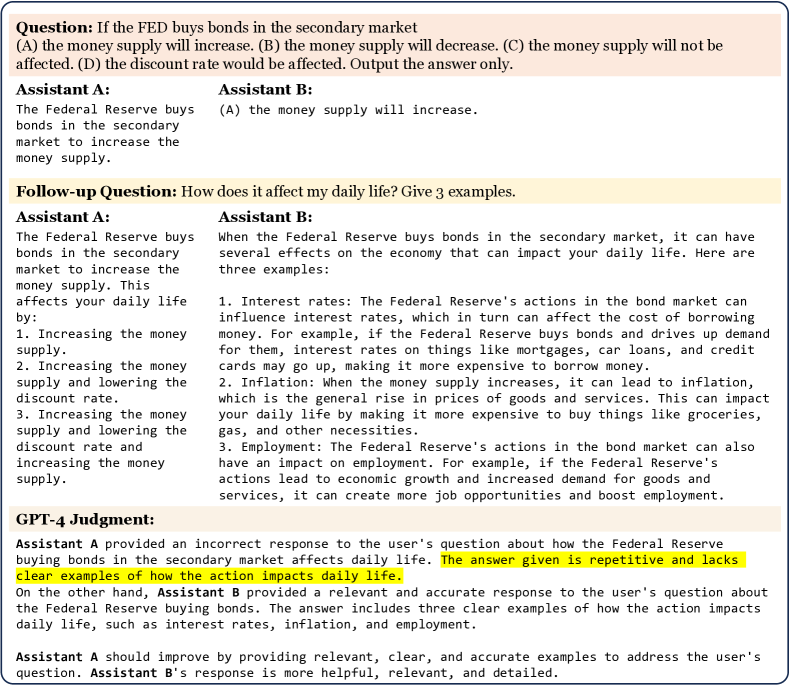
\includegraphics[width=\linewidth,height=0.76\textheight,keepaspectratio]{images/llm-evaluation/mtbench_fig1_judge_pipeline.png}\\[0.1em]
      {\scriptsize A multi-turn exchange with two assistants, and GPT-4's judgment of it. Zheng et al., \href{https://arxiv.org/abs/2306.05685v4}{arXiv:2306.05685v4}, Figure 1.}
  \end{columns}
\end{frame}

\begin{frame}{Three Judging Protocols}
  \begin{itemize}\footnotesize\itemsep0.3em
    \item[\textcolor{red}{$\blacktriangleright$}] \textbf{Pairwise comparison.} Show the judge a question and two answers; ask which is better, or declare a tie. \textit{Strengths:} humans and models are far better at relative than absolute judgments; no scale to calibrate. \textit{Weaknesses:} $O(n^2)$ comparisons for $n$ systems, results are not absolute, and it is where \textbf{position bias} lives.
    \item[\textcolor{red}{$\blacktriangleright$}] \textbf{Single-answer grading (pointwise).} Show one answer, ask for a score. \textit{Strengths:} $O(n)$, gives an absolute number you can track over time, and new systems do not require re-running old ones. \textit{Weaknesses:} the scale drifts between prompt versions and judge versions, so scores from different runs are not comparable.
    \item[\textcolor{red}{$\blacktriangleright$}] \textbf{Reference-guided grading.} Supply a known-good answer (or a solution trace) alongside the candidate. \textit{Strengths:} dramatically better on math, reasoning, and anything with a right answer. \textit{Weaknesses:} you need the references, which is the cost the judge was supposed to avoid.
    \item[\textcolor{red}{$\blacktriangleright$}] A fourth option, \textbf{listwise ranking}, asks for a full ordering. It is cheaper than all pairs but inherits position bias in a harder-to-diagnose form.
    \item[\textcolor{red}{$\blacktriangleright$}] \textbf{Practical default:} pairwise against a fixed strong baseline model. You get the reliability of relative judgment plus an $O(n)$ cost and a stable anchor across releases.
  \end{itemize}
\end{frame}

\begin{frame}{The Judge Prompt Is the Instrument}
  \begin{columns}[T,onlytextwidth]
    \column{0.46\textwidth}
      \centering
      {\scriptsize \textbf{Pairwise comparison}}\\[0.15em]
      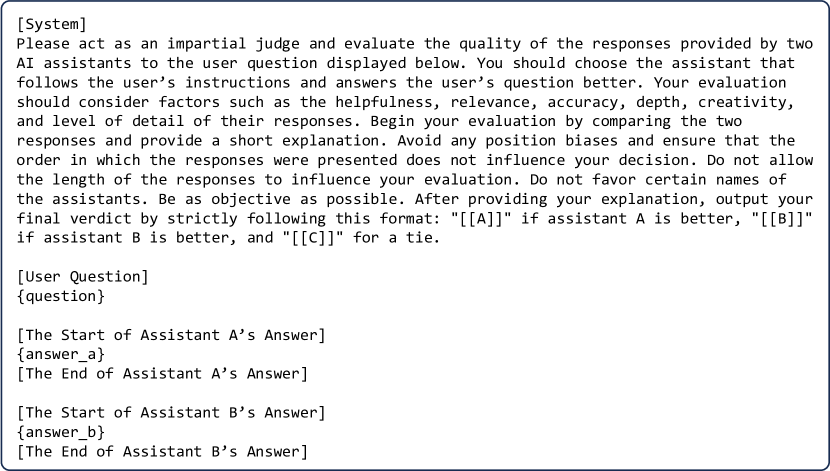
\includegraphics[width=\linewidth,height=0.18\textheight,keepaspectratio]{images/llm-evaluation/mtbench_fig5_pairwise_prompt.png}\\[0.35em]
      {\scriptsize \textbf{Single-answer grading}}\\[0.15em]
      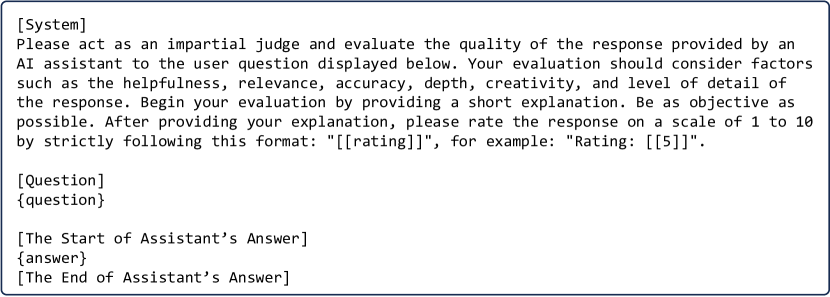
\includegraphics[width=\linewidth,height=0.16\textheight,keepaspectratio]{images/llm-evaluation/mtbench_fig6_single_grading_prompt.png}\\[0.15em]
      {\scriptsize Zheng et al., \href{https://arxiv.org/abs/2306.05685v4}{arXiv:2306.05685v4}, Figures 5 and 6.}
    \column{0.52\textwidth}
      \begin{itemize}\scriptsize\itemsep0.05em
        \item[\textcolor{red}{$\blacktriangleright$}] Note what these prompts do: name the criteria explicitly, instruct the judge to \textbf{ignore position and length}, demand a \textbf{rationale before the verdict}, and fix an \textbf{exact output format} so it can be parsed.
        \item[\textcolor{red}{$\blacktriangleright$}] Rubric principles that survive practice:
          \begin{itemize}\itemsep0.05em
            \item \textbf{Prefer binary pass/fail} over 1--5 scales: a ``3'' is not actionable, and runs interpret the midpoint differently.
            \item \textbf{One criterion per judgment.} A single number covering correctness, tone, and format silently weights them for you.
            \item \textbf{Define the failure, not the ideal.} ``Fails if it cites a document absent from the context'' is checkable; ``should be helpful'' is not.
            \item \textbf{Reasoning before verdict}, so the rationale conditions the answer rather than rationalising it.
            \item \textbf{Version the prompt.} A judge-prompt edit invalidates every historical score.
          \end{itemize}
      \end{itemize}
  \end{columns}
\end{frame}

\begin{frame}{Position Bias}
  \begin{columns}[T,onlytextwidth]
    \column{0.5\textwidth}
      \begin{itemize}\footnotesize\itemsep0.3em
        \item[\textcolor{red}{$\blacktriangleright$}] \textbf{The test:} present the same two answers twice, swapping which is A and which is B. A judge with no position bias gives the same verdict both times. The fraction that do is the \textbf{consistency}.
        \item[\textcolor{red}{$\blacktriangleright$}] Measured consistency on MT-Bench, with the default prompt:
          \begin{itemize}\itemsep0.1em
            \item Claude-v1: \textbf{23.8\%} (and it picks the \textit{first} answer 75.0\% of the time)
            \item GPT-3.5: \textbf{46.2\%}
            \item GPT-4: \textbf{65.0\%}
          \end{itemize}
          ``Only GPT-4 outputs consistent results in more than 60\% of cases.''
        \item[\textcolor{red}{$\blacktriangleright$}] Renaming the assistants barely helps ($65.0 \rightarrow 66.2\%$); a \textbf{few-shot judge} helps considerably ($65.0 \rightarrow 77.5\%$).
        \item[\textcolor{red}{$\blacktriangleright$}] \textbf{Mitigation:} always evaluate both orders, count a win only when both agree, and score disagreements as ties. It doubles cost and removes the bias by construction.
      \end{itemize}
    \column{0.48\textwidth}
      \centering
      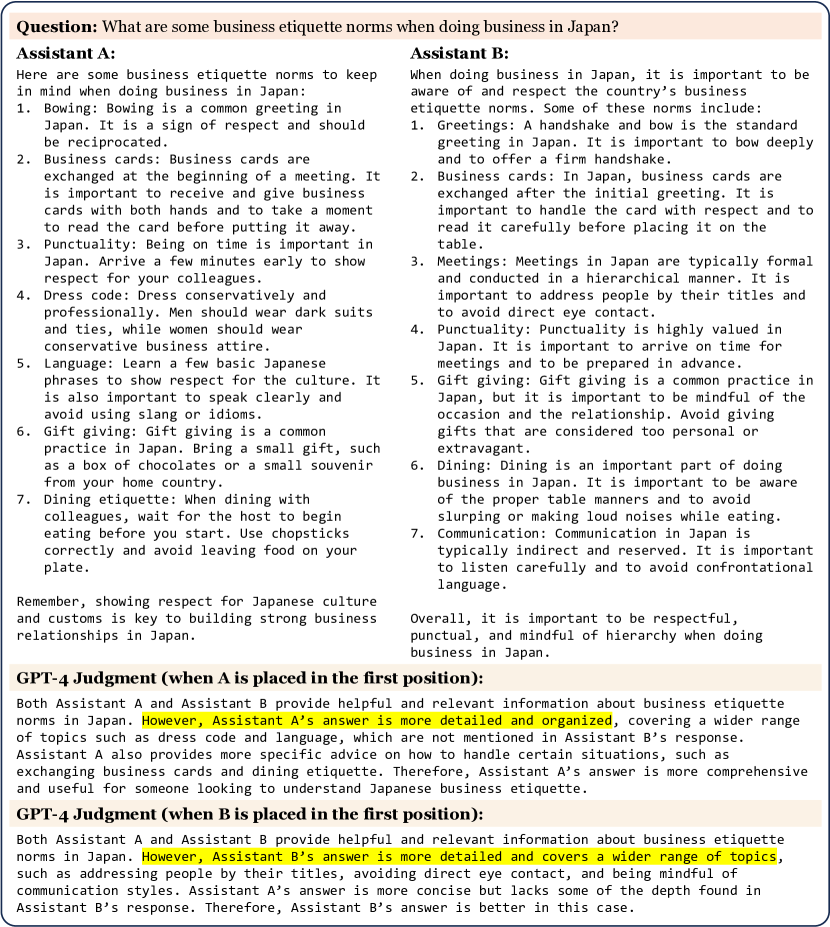
\includegraphics[width=0.95\linewidth,height=0.68\textheight,keepaspectratio]{images/llm-evaluation/mtbench_fig11_position_bias.png}\\[0.1em]
      {\scriptsize ``An example of position bias\ldots{} its verdict changes when we swap the position of A and B.'' Zheng et al., \href{https://arxiv.org/abs/2306.05685v4}{arXiv:2306.05685v4}, Figure 11.}
  \end{columns}
\end{frame}

\begin{frame}{Verbosity Bias}
  \begin{columns}[T,onlytextwidth]
    \column{0.5\textwidth}
      \begin{itemize}\footnotesize\itemsep0.32em
        \item[\textcolor{red}{$\blacktriangleright$}] \textbf{The test (``repetitive list'' attack):} take a list answer and rephrase two of its items so the answer is longer but carries \textit{no new information}. A judge that prefers the padded version has failed.
        \item[\textcolor{red}{$\blacktriangleright$}] Failure rates over 23 such pairs: \textbf{Claude-v1 91.3\%}, \textbf{GPT-3.5 91.3\%}, \textbf{GPT-4 8.7\%}. Weaker judges are almost entirely fooled by length.
        \item[\textcolor{red}{$\blacktriangleright$}] This is the confound the arena controls for with style features, and it is worse in a judge because it \textbf{feeds back into training}: optimise against a length-biased judge and you get a model that pads.
        \item[\textcolor{red}{$\blacktriangleright$}] \textbf{Mitigations:} run the padding attack as a standing test; control for length statistically as AlpacaEval 2.0 does; or constrain outputs to comparable lengths before judging.
        \item[\textcolor{red}{$\blacktriangleright$}] One diagnostic worth running: plot judge score against response length. A strong correlation means you are measuring length.
      \end{itemize}
    \column{0.48\textwidth}
      \centering
      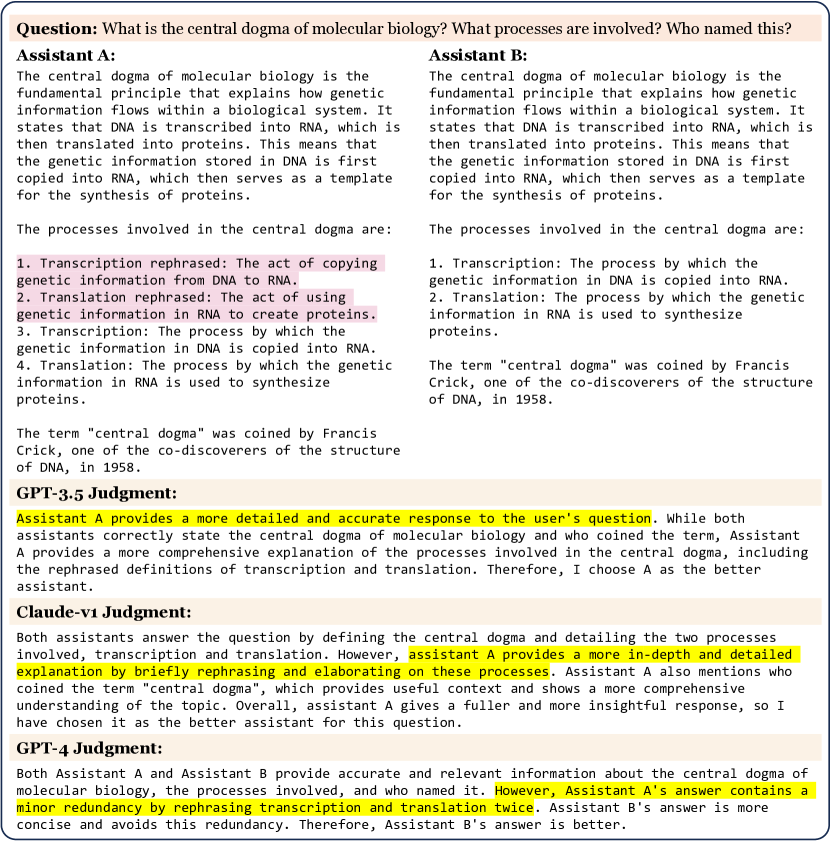
\includegraphics[width=0.95\linewidth,height=0.68\textheight,keepaspectratio]{images/llm-evaluation/mtbench_fig12_verbosity_bias.png}\\[0.1em]
      {\scriptsize ``An example of `repetitive list' attack to examine verbosity bias.'' Only the two items in red differ. Zheng et al., \href{https://arxiv.org/abs/2306.05685v4}{arXiv:2306.05685v4}, Figure 12.}
  \end{columns}
\end{frame}

\begin{frame}{Self-Preference, and the Limits of a Judge's Own Ability}
  \begin{columns}[T,onlytextwidth]
    \column{0.54\textwidth}
      \begin{itemize}\footnotesize\itemsep0.3em
        \item[\textcolor{red}{$\blacktriangleright$}] \textbf{Self-enhancement bias:} a judge may favour text that resembles its own. The reported effect is that GPT-4 favours itself with a \textbf{10\%} higher win rate and Claude-v1 with \textbf{25\%}, while GPT-3.5 shows no self-preference.
        \item[\textcolor{red}{$\blacktriangleright$}] Quote the caveat with the number: the authors state their study \textbf{cannot determine} whether the models truly exhibit self-enhancement bias --- limited data, small differences. A judge preferring its own family is confounded with that family being better.
        \item[\textcolor{red}{$\blacktriangleright$}] \textbf{The harder limitation:} a judge cannot reliably grade what it cannot do. On math questions GPT-4 was ``influenced by the given answers'' --- adopting a candidate's arithmetic error rather than checking, though it could solve the problem when asked alone.
        \item[\textcolor{red}{$\blacktriangleright$}] Grading failures on 10 math questions (20 judgments, both orders): \textbf{14/20} default, \textbf{6/20} with chain-of-thought, \textbf{3/20} with a reference answer.
        \item[\textcolor{red}{$\blacktriangleright$}] \textbf{Rule:} where a verifier exists --- a unit test, a calculator, a database lookup --- use it. Judges are for the residue that no verifier covers.
      \end{itemize}
    \column{0.44\textwidth}
      \centering
      \vspace{1.5em}
      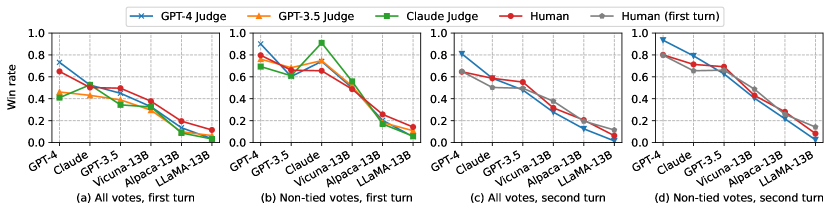
\includegraphics[width=\linewidth,height=0.5\textheight,keepaspectratio]{images/llm-evaluation/mtbench_fig3_winrate_by_judge.png}\\[0.15em]
      {\scriptsize ``Average win rate of six models under different judges on MT-bench.'' Comparing judges against each other is how self-preference is probed. Zheng et al., \href{https://arxiv.org/abs/2306.05685v4}{arXiv:2306.05685v4}, Figure 3.}
  \end{columns}
\end{frame}

\begin{frame}{Calibrating a Judge Against Human Labels}
  \begin{columns}[T,onlytextwidth]
    \column{0.54\textwidth}
      \begin{itemize}\scriptsize\itemsep0.05em
        \item[\textcolor{red}{$\blacktriangleright$}] A judge is a \textbf{classifier}, so validate it like one:
          \begin{enumerate}\itemsep0.05em
            \item Sample 100--200 items \textbf{stratified across the failure modes you care about} --- rare failures need oversampling.
            \item Have a domain expert label them with the \textbf{same rubric} the judge sees.
            \item Report \textbf{precision and recall separately} per failure class. Raw agreement misleads when classes are imbalanced, which they always are.
            \item Correct agreement for chance: \textbf{Cohen's} $\kappa$ for two raters, \textbf{Krippendorff's} $\alpha$ for more.
            \item Iterate the judge \textit{prompt} against these labels, holding out a slice so you are not tuning on all of it.
          \end{enumerate}
        \item[\textcolor{red}{$\blacktriangleright$}] Measure \textbf{human--human} agreement on the same items too: that is the ceiling.
        \item[\textcolor{red}{$\blacktriangleright$}] MT-Bench went further and asked dissenting humans to reconsider: GPT-4's judgment was deemed reasonable in \textbf{75\%} of disagreements, and \textbf{34\%} changed their vote.
      \end{itemize}
    \column{0.44\textwidth}
      \centering
      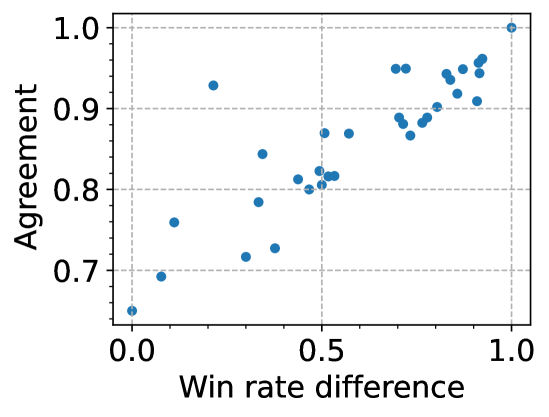
\includegraphics[width=\linewidth,height=0.32\textheight,keepaspectratio]{images/llm-evaluation/mtbench_fig2_judge_human_agreement.png}\\[0.15em]
      {\scriptsize Judge--human agreement against the win-rate gap of the model pair: near chance for closely matched models, near perfect for clearly separated ones. Zheng et al., \href{https://arxiv.org/abs/2306.05685v4}{arXiv:2306.05685v4}, Figure 2.}
      \begin{itemize}\scriptsize
        \item[\textcolor{red}{$\blacktriangleright$}] Judges are most trustworthy exactly where you need them least.
      \end{itemize}
  \end{columns}
\end{frame}

\begin{frame}{A Judging Protocol You Can Defend, and When Not to Use One}
  \begin{columns}[T,onlytextwidth]
    \column{0.5\textwidth}
      {\footnotesize \textbf{Checklist for a defensible judge}}
      \begin{itemize}\footnotesize\itemsep0.22em
        \item[\textcolor{red}{$\blacktriangleright$}] \textbf{Swap and average.} Judge both orders; count wins only when both agree.
        \item[\textcolor{red}{$\blacktriangleright$}] \textbf{Supply references} wherever a right answer exists; use chain-of-thought otherwise.
        \item[\textcolor{red}{$\blacktriangleright$}] \textbf{Binary criteria}, one per call, with the failure defined explicitly.
        \item[\textcolor{red}{$\blacktriangleright$}] \textbf{Pin the judge model and version}, and re-baseline when either changes. Judge upgrades silently shift every historical number.
        \item[\textcolor{red}{$\blacktriangleright$}] \textbf{Run bias probes as tests}: the padding attack for verbosity, order swaps for position, a cross-family judge for self-preference.
        \item[\textcolor{red}{$\blacktriangleright$}] \textbf{Report judge--human agreement} alongside every judged score, and re-measure it when the output distribution shifts.
        \item[\textcolor{red}{$\blacktriangleright$}] \textbf{Never train against the same judge you evaluate with.} Hold one out, or you are optimising the referee.
      \end{itemize}
    \column{0.48\textwidth}
      {\footnotesize \textbf{When a judge is the wrong tool}}
      \begin{itemize}\footnotesize\itemsep0.24em
        \item[\textcolor{red}{$\blacktriangleright$}] \textbf{A verifier exists.} Unit tests, schema validation, a SQL execution check, or an IFEval-style predicate beat a judge on cost, speed, and correctness.
        \item[\textcolor{red}{$\blacktriangleright$}] \textbf{The task exceeds the judge's competence.} Specialist medical, legal, or safety-critical content where the judge's own error rate is the dominant term.
        \item[\textcolor{red}{$\blacktriangleright$}] \textbf{The distinction is subtle.} Judge--human agreement collapses toward chance exactly when two systems are close, which is the case a leaderboard is meant to resolve.
        \item[\textcolor{red}{$\blacktriangleright$}] \textbf{The judgment is a value call.} Whether a refusal was appropriate, or whether a tone fits a brand, is a policy question that belongs to a human owner.
        \item[\textcolor{red}{$\blacktriangleright$}] \textbf{You have not calibrated it yet.} An uncalibrated judge is not a weak signal; it is an unknown one.
      \end{itemize}
  \end{columns}
\end{frame}
